
\section*{Materials and Methods: Illustrative Case Study}

\subsubsection*{Case Selection and Preparation}

To demonstrate the utility of the unified framework, we applied the KSS decomposition model to diagnostic decisions from 20 board-certified epileptologists evaluating 50 clinical cases. This case study is illustrated in Figure~\ref{Fig3-KSS}. The 50 clinical cases were from adult and pediatric patients presenting with suspected seizure(s), selected from the archives of four academic tertiary epilepsy centers in the United States. To ensure a robust reference standard, all cases had an established clinical diagnosis confirmed by either (i) habitual events captured on video-EEG during an epilepsy monitoring unit (EMU) admission or (ii) a minimum of 6 months of clinical follow-up.

The case mix was intentionally balanced to represent a spectrum of case difficulty typical of a subspecialty practice:
\begin{itemize}
    \item \textbf{Prevalence:} The cohort included 25 epilepsy cases and 25 non-epilepsy cases.
    \item \textbf{Difficulty:} Cases were categorized by the authors into four difficulty bins (easy, moderate, difficult, and very difficult) to ensure a broad spectrum of diagnostic complexity.
    \item \textbf{Case Profiles:} Among epilepsy cases, 12 were confirmed by EEG and 13 by follow-up; among non-epilepsy cases, 6 were confirmed by EEG and 19 by follow-up.
\end{itemize}

\subsubsection*{Participants and Experimental Procedure}

Twenty board-certified multinational epileptologists from 18 academic centers across 5 countries were recruited to independently review the cases. Experts had an average of 20 years in practice (range: 2.5-40 years; median: 19 years). The experiment followed a three-step structured judgment process:

\begin{enumerate}
    \item \textbf{Initial Assessment (Question 1):} Experts reviewed a clinical vignette summarizing history and physical exam data and rated the likelihood of epilepsy as "low," "intermediate," or "high".

    \item \textbf{Supplemental Testing (Question 2):} If "intermediate" was selected, experts were provided with a representative 10- to 20-second routine scalp EEG epoch and a summary of neuroimaging findings. They then provided a binary "yes/no" diagnosis.

    \item \textbf{Difficulty Rating (Question 3):} Experts rated the perceived difficulty of each case using a 5-point Likert scale.
\end{enumerate}

To measure occasion noise, the entire process was repeated after a washout period of at least 30 days.


\subsubsection*{Response Coding for Variance Decomposition}

For the noise decomposition analysis, we modeled responses to both questions as binary outcomes. For Question 1, we coded "high" probability (the expert believes the patient has epilepsy) as 1, while both "low" and "intermediate" were coded as 0. For Question 2, the responses were already binary ("yes" = 1, "no" = 0). This coding scheme allows us to apply the unified GLMM framework (Equation~\ref{eq:master-model}) to decompose variance into signal and noise components separately for each diagnostic stage.

\subsection*{Results}

\subsubsection*{Variability and Consistency}

Experts varied widely in their diagnostic thresholds and interpretations. The probability of receiving a different final diagnosis when seeing the same expert on different occasions was 16\% (162 diagnostic reversals out of 1,000 case evaluations). The probability of two different experts making a different diagnosis for the same case was 26\%. At the individual case level, the proportion of experts diagnosing epilepsy ranged from 0\% to 80\% across the 50 cases, with the number of experts requesting supplemental testing (EEG/neuroimaging) ranging from 4 to 20 per case.

\subsubsection*{Noise Decomposition}

\textbf{A Shift in Noise Profiles.} We applied the KSS model (Equation~\ref{eq:master-model}) to decompose variation in expert diagnoses. The framework reveals a fundamental shift in the source of disagreement when experts move from clinical history alone to a full diagnostic workup. Table~\ref{tab:variance-results} summarizes the variance components for both stages.

\begin{table}[h!]
\centering
\small
\begin{tabular}{lcccc}
\toprule
& \multicolumn{2}{c}{\textbf{Question 1 (History Only)}} & \multicolumn{2}{c}{\textbf{Question 2 (Final Diagnosis)}} \\
\cmidrule(lr){2-3} \cmidrule(lr){4-5}
\textbf{Component} & \textbf{Std. Dev ($\sigma$)} & \textbf{\% Variation} & \textbf{Std. Dev ($\sigma$)} & \textbf{\% Variation} \\
\midrule
\textbf{Signal ($c_i$)} & -- & 66\% & -- & 69\%  \\
\textbf{Level Noise ($\ell_j$)} & -- & 23\% & -- & 5\%  \\
\textbf{Pattern Noise ($p_{ij}$)} & -- & 10\% & -- & 24\%  \\
\textbf{Occasion Noise ($o_{ijt}$)} & -- & 1\% & -- & 1\%  \\
\midrule
\textbf{Total System Noise} & -- & 34\% & -- & 31\%  \\
\bottomrule
\end{tabular}
\caption{Variance decomposition of expert responses in epilepsy diagnosis. Percentages represent the proportion of total variation explained by each component on the latent (logit) scale. Question 1 was based on clinical history alone; Question 2 incorporated EEG and neuroimaging results.}
\label{tab:variance-results}
\end{table}

\textbf{Stage 1 (Clinical History Only):} Disagreement was primarily driven by \textit{level noise} (23\% of total variation). This suggests that in the absence of objective data, expert disagreement is a "threshold problem"---some experts are simply more inclined to diagnose epilepsy than others. 

\textbf{Stage 2 (Full Diagnostic Workup):} Once EEG and neuroimaging data were introduced, level noise decreased to 5\%, but \textbf{pattern noise} rose to 24\%. This indicates that supplemental testing "calibrates" experts' thresholds (reducing systematic bias) but introduces new idiosyncratic disagreements regarding the interpretation of specific test features. 

\textbf{Key findings from the variance decomposition:}

\begin{itemize}
    \item \textbf{Noise Magnitude:} Approximately one-third of the total variation in final expert diagnoses was attributable to noise (31-34\%).

    \item \textbf{The "Information Shift":} Providing additional diagnostic information (EEG/neuroimaging) reduced overall noise only modestly (from 34\% to 31\%), but \textit{shifted the dominant noise source}. The framework reveals that moving from subjective to objective data does not eliminate disagreement---it transforms it from a threshold problem (level noise) to an interpretation problem (pattern noise).

    \item \textbf{Expert Inconsistency:} While the probability of an expert disagreeing with their own previous diagnosis was 16\%, occasion noise only accounted for 1\% of the total variance. This suggests that diagnostic "flip-flopping" happens mostly when cases are inherently ambiguous or near the expert's decision threshold. 

    \item \textbf{Difficulty Impact:} Most noise and disagreement occurred in "difficult" cases, where expert agreement dropped to 50\%.
\end{itemize}

Figure~\ref{fig:variance-decomp} visualizes the variance decomposition across all three diagnostic stages. The Gaussian distributions illustrate the estimated magnitude of each variance component (signal and noise types), with tick marks showing the distribution of estimated random effects. The stacked bar charts quantify the relative contribution of each component to total variation. The dramatic shift in noise profile from Stage 1 to Stage 2 is immediately apparent: level noise (medium gray) shrinks from 23\% to 5\%, while pattern noise (light gray) expands from 10\% to 24\%, despite total system noise remaining nearly constant at approximately one-third of total variation.

\begin{figure}[h!]
\centering
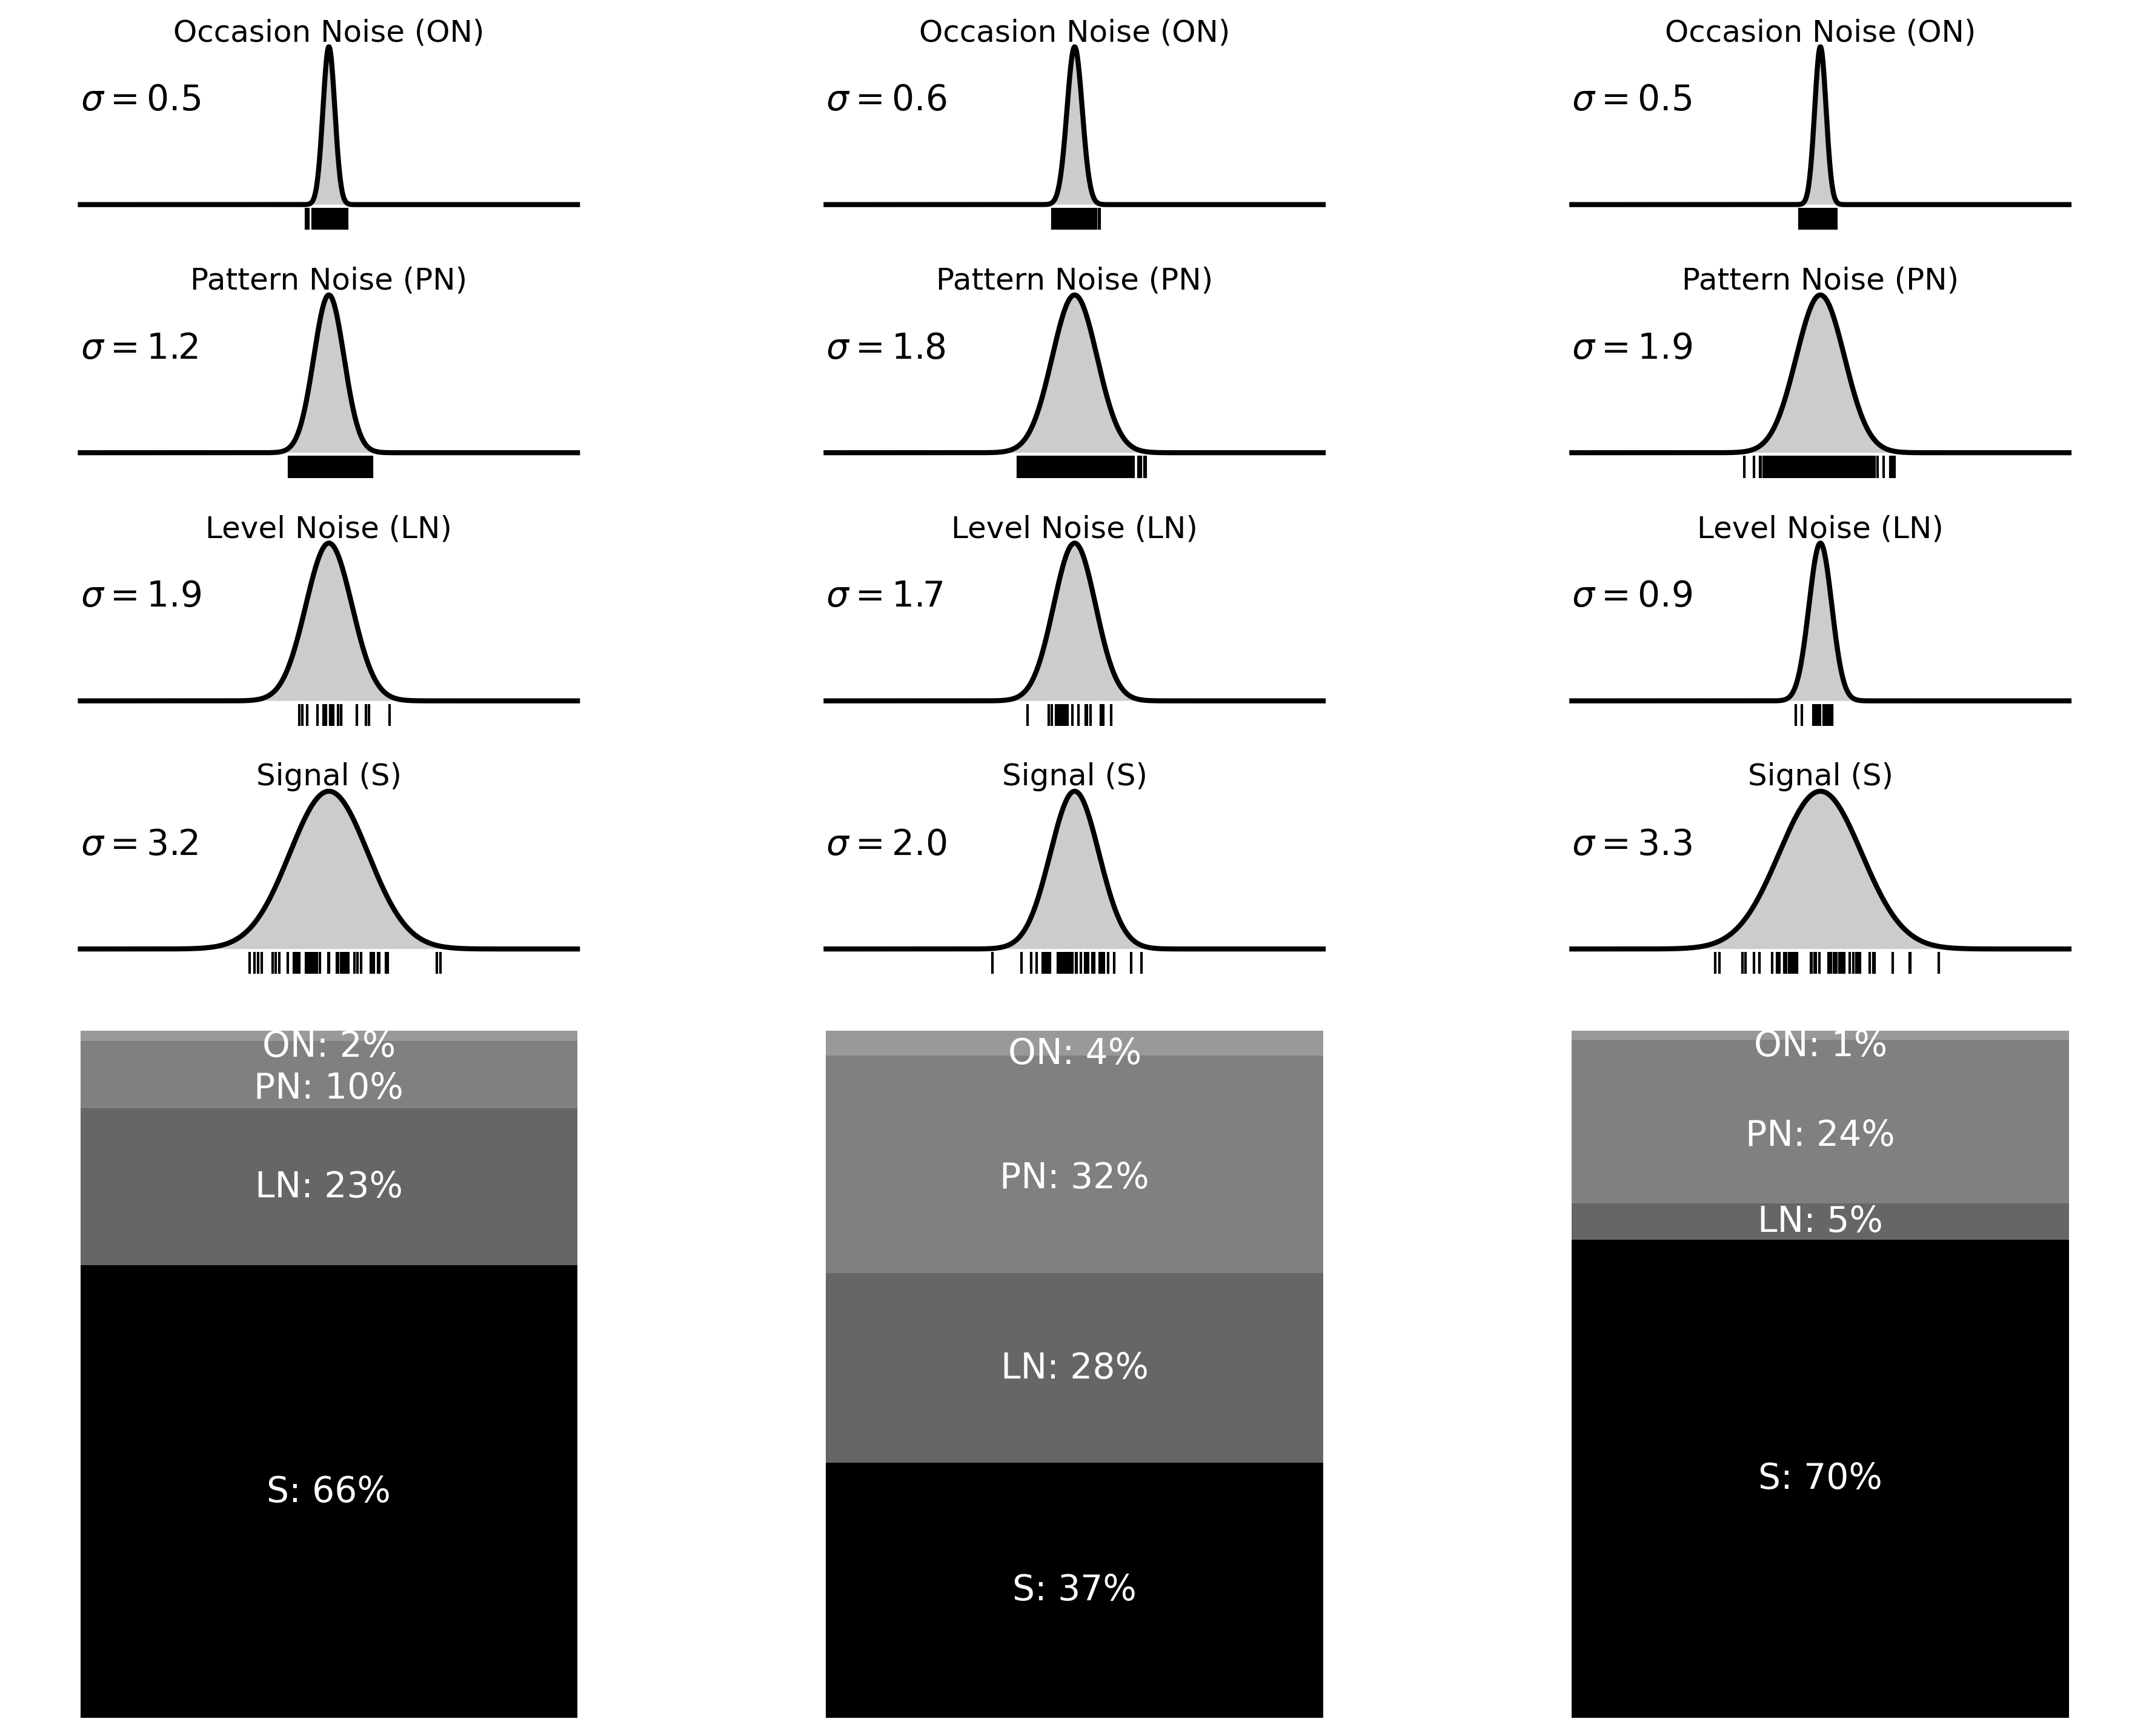
\includegraphics[width=0.95\textwidth]{Figure3.png}
\caption{Variance decomposition across three diagnostic stages in the epilepsy case study. Each column represents a different diagnostic stage: \textbf{Left:} Stage 1 (clinical history only); \textbf{Middle:} Decision to request supplemental testing; \textbf{Right:} Stage 2 (final diagnosis with EEG and neuroimaging). For each stage, Gaussian curves show the distribution of estimated variance components, with tick marks indicating individual random effect estimates. Stacked bar charts (bottom) display percentage contributions to total variation. S = signal (case difficulty); LN = level noise (systematic expert threshold differences); PN = pattern noise (idiosyncratic case interpretation); ON = occasion noise (within-expert inconsistency). Note the "information shift": adding objective tests (Stage 1 to Stage 2) reduces level noise (23\% $\rightarrow$ 5\%) but increases pattern noise (10\% $\rightarrow$ 24\%), transforming disagreement from a threshold problem to an interpretation problem.}
\label{fig:variance-decomp}
\end{figure}

\subsubsection*{Diagnostic Accuracy}

Mean accuracy relative to the clinical diagnosis was 60\% after Question 1 (range across experts: 50-70\%) and 71\% after the final diagnosis incorporating test results (range: 63-81\%). Accuracy varied substantially with case difficulty. For cases rated as easy or moderate by study authors, mean accuracy was 87\%, while for difficult and very difficult cases, accuracy dropped to 56\%. Among cases rated as easy by experts during the study, mean accuracy was 92\%, whereas cases rated as neither easy nor difficult had mean accuracy of 64\%.

Notably, diagnostic accuracy did not significantly correlate with years of practice (r = 0.18, p = 0.46), suggesting that experience alone does not eliminate noise. This underscores the need for systematic approaches to improve diagnostic reliability beyond simply accumulating clinical experience. 

\subsection*{Intervention Roadmap: From Measurement to Action}

The primary value of decomposing noise into distinct types is that each suggests different remedies. Table~\ref{tab:intervention-roadmap} maps the mathematical output of the model to specific quality improvement actions.

\begin{table}[h]
\centering
\caption{Intervention roadmap: Mapping noise types to targeted quality improvement strategies}
\label{tab:intervention-roadmap}
\begin{tabular}{@{}p{0.2\textwidth}p{0.3\textwidth}p{0.4\textwidth}@{}}
\toprule
\textbf{If the model shows high...} & \textbf{It means...} & \textbf{Recommended Intervention} \\
\midrule
\textbf{Level Noise} ($\sigma_\ell^2$) &
Experts have systematically different diagnostic thresholds (some are more conservative, others more liberal). &
\begin{itemize}[leftmargin=*, nosep]
    \item Threshold calibration exercises with known-difficulty cases
    \item Standardized diagnostic guidelines with explicit criteria
    \item Feedback on personal diagnostic tendencies
\end{itemize} \\
\midrule
\textbf{Pattern Noise} ($\sigma_p^2$) &
Experts interpret the same case features differently (e.g., disagreement on what constitutes a "significant" EEG spike). &
\begin{itemize}[leftmargin=*, nosep]
    \item Case-based group training sessions with discussion of discordant cases
    \item AI-assisted feature detection to standardize measurements
    \item Develop shared mental models through deliberate practice
\end{itemize} \\
\midrule
\textbf{Occasion Noise} ($\sigma_o^2$) &
Individual experts are inconsistent over time (fatigue, mood, time-of-day effects). &
\begin{itemize}[leftmargin=*, nosep]
    \item Decision support tools that prompt consistency checks
    \item "Second-read" protocols for borderline cases
    \item Workflow scheduling to minimize fatigue effects
\end{itemize} \\
\bottomrule
\end{tabular}
\end{table}

\subsection*{Interpreting the Shift: A Guide for Quality Improvement}

The epilepsy case study illustrates why traditional reliability metrics are insufficient for guiding interventions. A conventional analysis using Cohen's kappa would show modest improvement in agreement from Stage 1 to Stage 2, leading to the conclusion that "adding EEG and neuroimaging improves diagnostic reliability." While technically true, this misses the actionable insight.

\textbf{What traditional metrics would show:}
\begin{itemize}
    \item Stage 1 (History): Fair agreement (Fleiss' kappa = 0.33)
    \item Stage 2 (History + EEG/Imaging): Moderate agreement (Fleiss' kappa = 0.52)
    \item Conclusion: "EEG improves reliability"
\end{itemize}

However, these summary statistics conceal substantial heterogeneity. Pairwise Cohen's kappa between individual expert pairs ranged from $-0.06$ to $1.00$ in Stage 1 (mean = 0.27, SD = 0.27) and from $0.09$ to $0.84$ in Stage 2 (mean = 0.52, SD = 0.14). The dramatic reduction in variability (SD decreased by nearly half) indicates that objective testing not only improves average agreement, but also reduces the dispersion of agreement across expert pairs---some pairs of experts who strongly disagreed on clinical history alone achieved moderate agreement once test results were available.

\textbf{What the noise decomposition reveals:}
\begin{itemize}
    \item Stage 1: The disagreement is primarily a \textbf{Rater Problem} (Level Noise = 23\%). Different experts have different thresholds for what constitutes "sufficient evidence" for epilepsy diagnosis.
    \item Stage 2: The disagreement transforms into a \textbf{Feature Interpretation Problem} (Pattern Noise = 24\%). Experts now agree on general thresholds, but disagree on how to interpret specific EEG morphologies or imaging findings.
\end{itemize}

\textbf{Implications for quality improvement:}
\begin{itemize}
    \item \textit{Wrong intervention:} A quality improvement team using only kappa might conclude "we need more testing" or "we need better tests."
    \item \textit{Correct intervention:} The framework reveals that Stage 1 requires \textbf{threshold calibration} (e.g., anchoring vignettes, consensus guidelines on diagnostic thresholds), while Stage 2 requires \textbf{feature standardization} (e.g., EEG morphology atlases, inter-rater training on spike classification, AI-assisted feature detection).
\end{itemize}

This is the core value proposition of the framework: it transforms reliability measurement from a descriptive statistic into a diagnostic tool that identifies \textit{which} intervention will be most effective at each stage of the diagnostic process.

